% #############################################################################
% This is Chapter 3
% !TEX root = ../main.tex
% #############################################################################
\fancychapter{Hybrid models for children automatic speech recognition}
\label{chap:Chapter3}
\cleardoublepage
\section{Introduction}
% Why HMM-DNN for children
In Chapter \ref{chap:Chapter2}, we saw how a HMM-GMM or HMM-DNN ASR system may integrate knowledge into the automatic speech recognition pipeline. It uses knowledge from language model, acoustic model, and vocabulary to reduce the amount of speech data required to generate appropriate results. According to the literature, these results can be further improved with inductive bias approaches such as transfer learning and multi-task learning \cite{TransferLF}. For years, hybrid configurations have been a privileged setting for the children's ASR community. As a matter of fact, between 2009 and 2020, 80\% of published research on children's speech recognition was based on hybrid systems, with 45\% using HMM-GMM and 35\% HMM-DNN. However, during the same period, 63\% of published work was conducted for English \cite{big_review_childASR}. As a result, it is uncertain how children's speech from other languages relates to the various approaches used in English, particularly transfer and multi-task learning.

% What we planned to do here
This chapter will investigate these strategies in a variety of scenarios employing non-English data. First, we present transfer and multi-task learning using adult speech as an inductive bias, as is common in the literature. Second, because there is a lack of data for both adult and children's low-resource languages, we investigate the same methodologies using only children's speech. Finally, we present our approach, multilingual transfer learning, which combines transfer and multi-task learning to produce a more robust model for speech recognition in low-resource children setting.

\section{Multi-task and Transfer learning using adult and children data}
\label{section:HMMDNNADULT2CHILD}
\subsection{Methodology}

Motivated by the success of knowledge transfer approaches for ASR children using adult data in the research \cite{TFchildren,TransferLF,2019multi}, we intend to validate these findings using a low-resource language. Indeed, using adult data for pre-training makes sense since adult speech is more stable and less prone to variation. Using adult speech to train a speech recognition algorithm makes it simpler to extract and recognize intrinsic and meaningful speech patterns.

For this proposal, we assess children's speech recognition performances in four distinct configurations:
\begin{enumerate}
    \item \textbf{Adult model}: Using a model trained from scratch with only adult data.
    \item \textbf{Children model}: Using a model trained from scratch with only children data.
    \item \textbf{Multi-task model}: Using a model trained jointly on adult and children data in parallel using multi-task learning.
    \item \textbf{Transfer learning}: Using a model that has been fine-tuned on children data from the adult model of configuration 1.
    %\item \textbf{Transfer learning with well-resource corpus}:  Using a model that has been finetuned on children data from the adult model trained on large amount of adult English data.
\end{enumerate}

\subsection{Corpus}
\label{sec:corpus}
As stated in the introduction, we aim to evaluate the performance of children's speech in a low-resource language. To this end, we decided to use European Portuguese corpora. European Portuguese can be considered a low-resource language since most adult speech corpora do not exceed 100 hours \cite{tribus}.
In this experiment, we used LetsRead, a child corpus, described in section \ref{section:children_corpora} and BD-PUBLICO as adult corpus. %However, given the relatively small size of BD-PUBLICO, we chose to expand our experiments with a large English corpus, Librispeech-960. 
The statistics of all these two corpora are provided in the following table \ref{tab:statistics_exp1}. The rest of this section provides further information about the BD-PUBLICO corpus.%these two adult corpora.

% Stat corpus 
\begin{table}[h]
\begin{center}
\begin{tabular}{lcc}
\hline
Corpus name      & Train & Test  \\ \hline
\multicolumn{1}{l}{BD-PUBLICO}             & 8085 utt  & 412 utt  \\ 
\multicolumn{1}{c}{\textit{Adult}}              & 21h48 & 01h10 \\\hline
\multicolumn{1}{l}{LETSREAD}     & 3590 utt & 1039 utt \\ 
\multicolumn{1}{c}{\textit{Children}}     & 12h00 & 02h30 \\  \hline
%\multicolumn{1}{l}{Librispeech}                     & 281241 utt &   \\ 
%\multicolumn{1}{l}{}      &                &  960h &  \\ \hline
\end{tabular}
\caption{Number of utterances and duration of the different corpora for multi-task and transfer learning experiments using adult and children data}
\label{tab:statistics_exp1}
\end{center}
\end{table}

\subsubsection*{BD-PUBLICO}
The BD-PUBLICO database (Base de Dados em Português eUropeu, vocaBulário Largo, Independente do orador e fala COntínua) \cite{bdpublico} consists of reading sentences extracted from Portuguese newspaper PÚBLICO. The sentences that are read correspond to a total of 6 months of news (equivalent to 10M words and 156k different forms). It is composed of 120 speakers, and graduate and undergraduate students from Instituto Superior Técnico (Lisbon). This corpus is considered an adult dataset since all students are between 19 and 28 years old. All recordings were performed in good noise condition, in a soundproof room at INESC-ID (Lisbon), at a sampling frequency of 16kHz and using a high-quality microphone. In addition, a pronunciation lexicon with citation phonemic transcriptions for each word was produced. Finally, manually corrections were applied to the automatically generated transcriptions. 

We divided the BD-PUBLICO corpus into three unique sets with balanced gender partitioning: 1) A training set of 80 sentences by 100 speakers. 2) A development set of 40 sentences performed by a total of 10 speakers. Finally, a test set of 40 sentences by 10 speakers.

%\subsubsection*{Librispeech}
%Librispeech corpus is one of the biggest publicly available speech dataset \cite{librispeech}. It is a collection of 982 hours recorded at 16kHz from 2484 adult speakers derived from audiobooks. Librispeech corpus is designed to ensure a gender balance and no speaker overlap between train, development and test sets.


\subsection{Experimental setup}
\label{section:exp_setup}

All experiments were carried out using the Kaldi open-source toolkit \cite{kaldi}. First, for each corpus, an independent HMM-GMM acoustic model was trained to produce the necessary alignment for the HMM-DNN model. Then, HMM-DNN acoustic models were trained using  40-dim filter-banks (fbanks) in addition to a 40-dim Spectral Subband Centroid (SSC) features \cite{ssc}. These features are known to have similar properties to formant frequencies. Thus, we expect them to help vowel recognition and lead to better recognition of children's speech. 
The resulting 80-dim input features are then augmented by a 100-dim i-vector. Concatenating speaker embeddings to the input features helps to improve model speaker robustness \cite{ivector}. For our experiments, we use an i-vector extractor trained on a set of pooled children data from different languages.

Data augmentation was applied to all training corpora by perturbing the speaking rate of each training utterance by 0.9 and 1.1 factors; as well as volume perturbation. This helps the network to be more robust to rate and volume variability on the test sets. To further improve the robustness of the model, Specaugment \cite{specaugment}  was applied on top of the fbanks and SSC features by randomly masking time and frequency bands.

For all experiments, we kept the same HMM-DNN acoustic model architecture using lattice-free maximum mutual information (LF-MMI) objective with a learning rate of 2.0E-4. The acoustic model architecture is divided into two parts: i) six convolutional neural network layers and seven TDNN-F layers of dimension 1024  and followed by ii) two TDNN layers of dimension 450 and a fully-connected layer.

For the transfer learning experiments, only the first part of the network will be fine-tuned, while the second part will be dropped and replaced by randomly initialized ones. Similarly, for the multi-task learning experiment, the first part will be shared between the adult and the child, while the second part will be independent.



\subsection{Results}
\begin{table}[h]
\centering
\begin{tabular}{c|ccc}
\hline
 Method & Adult WER $\downarrow$   & Children WER  $\downarrow$   \\ \hline
\multicolumn{1}{c|}{Adult model} & 3.82\%   &  102.83\%\\ 
\multicolumn{1}{c|}{Children model} & 45.56\%  & 26.88\% \\ 
\multicolumn{1}{c|}{Multi-task model}  &   4.59\% &  27.65\% \\ 
\multicolumn{1}{c|}{Transfer learning} &  -  & 25.36\% \\ \hline
%\multicolumn{1}{c|}{Transfer learning from Librispeech} & -  & 25.18\% \\ \hline


\end{tabular}

\caption{WER results using adult data for knowledge transfer methods}
\label{tab:res_exp1}
\end{table}

% Adult model
The WER scores for all settings are presented in table \ref{tab:res_exp1}. In the first row, we notice that employing a model trained on adult data yields a WER of 102.83\% on the children's test set. This model achieves 3.82\% for BD-PUBLICO. This degradation in the children's compared to adults' scores demonstrates the presence of considerable variability in children's speech, which has a detrimental impact on the ASR scores. It supports the idea that an acoustic model designed exclusively for children is necessary because child speech is currently unusable with adult systems.

% Children model
Training the acoustic model directly on the children's data, on the other hand, considerably improved the word error rate on the children's data to 26.88\%. Since the model observes acoustic variability during training, it becomes more robust to it. While the model improved for children, it deteriorated adult speech recognition performance to 45.56 \% WER. This confirms the acoustic mismatch between adult and children speech once more. We compare transfer and multi-task learning approaches using these two experiments as a baseline.

% Multi-task
When the model was trained jointly utilising adult and children data in the scenario of multi-task learning, the recognition score of the adults and children decreased marginally when compared to the adult and child model baselines. Unlike in the adult and child models, where the mismatch significantly reduced the children's score in the adult model and the adult's score in the child model, both recognition scores in this multi-task learning scenario are comparable to their respective "trained from scratch" baselines. These results were achieved by including corpus-specific layers into the acoustic model architecture. 
Indeed, the model's shared component will learn the key characteristics of Portuguese speech, while the corpus-specific part will focus on how to apply them to adults and children, respectively.

% TL BD-Publico
In the fourth line, Training over children data with a pre-trained Portuguese adult model as initialization enhanced the result to 25.36\% WER. When compared to weights random initialization, it is shown that the weights of the adult model are a beneficial starting configuration and allow the transfer learning model to learn relevant patterns for children. It avoids the need for the model to learn these patterns from scratch, using data from a highly variable source. As a result, transfer learning may be considered a viable strategy for improving the ASR performance for children's speech. This finding is consistent with the literature on hybrid models\cite{TransferLF,TFchildren}. 

% TL Librispeech
%Finally, employing transfer learning from well-resourced but out-of-domain speech data, here Librispeech, improves recognition scores for Portuguese children, with a 25.18\% WER. When compared to weights random initialization, it shown that the weights of the English model are a beneficial starting configuration and allow the transfer learning model to attain learn relevant patterns for children.In the literature, similar behavior has been reported \cite{kunze2017transfer}.

\subsection{Summary and discussion}
% Conlusion
In this study, we conducted a knowledge transfer technique analysis to improve the results of ASR systems for children. We corroborate the acoustic mismatch between adult and child speech and the importance of the model encountering child data and its variability. Our investigations revealed that the transfer learning approach is a promising way to improve low-resource children's speech recognition scores. Furthermore, multi-task learning was found to be helpful in the setting of mixed adult-child ASR acoustic modelling.
% Open question for next section
However, in this study, we focus on the transfer from adults to children. It is not clear how such a system can work using only children's data.



\section{Multi-task and transfer learning using multilingual children data}
\subsection{Motivation}
% Explain motivation
In this section, we study whether the performance of children's ASR for low-resourced languages may be improved by combining children's resources from different languages. In many cases, there is limited or no data for both adults and children. Therefore, we propose using several small-sized corpora of children from various languages to overcome the substantial acoustic variability and data scarcity issues. The current study extends standard multilingual training and transfer learning for hybrid HMM-DNN ASR by combining them in a meaningful way to use knowledge from heterogeneous data. First, a multilingual model trained with a multi-task learning objective tries to optimise network parameters to the specific characteristics of children's speech in multiple languages/tasks simultaneously. Subsequently, this multilingual model is used to improve ASR for a target language --potentially different from those used in the multilingual training stage-- by using transfer learning. We address the following research question: Does this two-step training strategy outperform conventional single language/task training for 's speech, as well as multilingual and transfer learning alone?

\subsection{Proposed approach}
\label{section:method}
We propose to combine transfer learning (TL) and multi-task learning (MTL) together for improved acoustic modelling of hybrid HMM-DNN ASR.
The proposed approach consists of a two-stage procedure using both MTL and TL that extends the existing techniques since these are usually applied separately.
First, a multilingual model trained with a multi-task learning objective attempts to optimize the network parameters to the particular characteristics of children's speech in multiple languages in parallel. In this work, the model is considered multilingual because all the tasks trained during multitask learning are a corpus of children from different languages.
Secondly, we adapt this model for a specific children's corpus with TL. The motivation for using TL as a second stage is to take advantage of the robust pre-trained model trained during the MTL phase. Indeed, this pre-trained model has potentially learned cross-linguistic information about children's speech but has also seen more children's data than a model trained in a single language. 
For this purpose, the acoustic model is divided into two parts: the layers close to the input are shared across all languages and the top layers are language-specific. That is, there are as many output layers as there are languages, i.e. children corpora. Notice that one can incorporate a new language/task in this second stage by adding a new language-specific output,  even if this new language/task has not been seen during  MTL training (figure \ref{fig:MLTL1}).
%ICASSP-Thomas Remove equation related reference
%(see equation \ref{equation:MT}).
Our hypothesis is that the more data has been seen by the acoustic model, the better the shared layers can capture the underlying characteristics of children's speech during the first stage of the procedure. These characteristics can be used effectively, later,  by the language-specific layers and during the second step of the procedure (figure \ref{fig:MLTL1}). 

Although the approaches adopted in this work have been used previously in other studies, for instance \cite{TransferLF} and \cite{2019multi} where they successfully applied MTL using children speaking  Mandarin and English, obtaining a relative improvement of 16.96\% WER in the English children case, it is clear that successful performance of a methodological approach in the case of English cannot be expected to generalize to other contexts and languages.  
As we all know, English is a large-size, resource-rich pluricentric language which should be seen more as an exceptional case, rather than an average representative. Against this background, it is important to emphasize that there is a need for research that investigates whether methods that have already been tested for English also work in new contexts such as those of mid-sized languages with fewer resources than English, like Dutch, Portuguese, Swedish and German. 
\begin{figure}[t]
\begin{center}
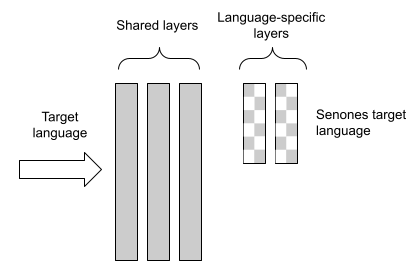
\includegraphics[scale=0.5]{imgs/Ours_final.png}
\caption{Multilingual transfer learning approach. Language-specific layers can be randomly initialized for a language not present during the MTL phase or use the corresponding pre-trained layers in case the target language was present during the MTL phase. Grey blocks are pre-trained during MTL phase.}
\label{fig:MLTL1}
\end{center}
\end{figure}


\subsection{Setup}
\label{section:corpus}
All experiments were conducted using five children corpora, each from a different language. Namely PFSTAR\_SWE, ETLTDE, CMU, LETSREAD and CHOREC. All those datasets have been described in section \ref{section:children_corpora}.%This section briefly presents each corpus and how it was used in the present study. In addition, more 
Table \ref{tab:statistics} presents statistics about the duration, number of utterances and language %can be found in Table \ref{tab:statistics}. 
Notice that in this work we have only used small datasets to better reflect the average size of the available children's speech corpora.

\begin{table}[ht]
\begin{center}
\begin{tabular}{llcc}
\hline
Corpus name & Language     & Train & Test  \\ \hline
\multicolumn{1}{l}{PFSTAR\_SWE} & Swedish             & 6030 utt  & 2879 utt  \\ 
\multicolumn{1}{l}{} &              & 04h00 & 01h48 \\\hline
\multicolumn{1}{l}{ETLTDE}      & L2 German   & 1445 utt &  339 utt \\ 
\multicolumn{1}{l}{}      &    &  04h41 & 01h06 \\ \hline
\multicolumn{1}{l}{CMU}         & English             & 3637 utt & 1543 utt \\ 
\multicolumn{1}{l}{}         &              & 06h26 & 02h45  \\ \hline
\multicolumn{1}{l}{LETSREAD}    & Portuguese & 3590 utt & 1039 utt \\ 
\multicolumn{1}{l}{}    &  & 12h00 & 02h30 \\  \hline
\multicolumn{1}{l}{CHOREC}      & Dutch               & 2490 utt & 575 utt  \\ 
\multicolumn{1}{l}{}      &                &  20h12 & 04h42 \\ \hline
\end{tabular}
\caption{Statistics on the different corpora of children's speech.}
\label{tab:statistics}
\end{center}
\end{table}

We employ the same experimental design as the prior experiment with adult data from section \ref{section:exp_setup} setup, where the acoustic model is divided in two. The first part is shared across all languages, whereas the second is language specific.
Furthermore, each corpus, i.e. each language, uses an independent language model and lexicon that is constant throughout all experiments in order to assess solely the acoustic model contribution.

\subsection{Multilingual-transfer learning experiment}

\begin{table*}[ht] 
\begin{center}
\begin{small}
\begin{tabular}{c|ccccc}

\hline
 & PFSTAR\_SWE & ETLTDE & CMU &  LETSREAD & CHOREC   \\  \hline
 \multicolumn{1}{c|}{Language} & \textit{Swedish} & \textit{German}  &  \textit{English}  & \textit{Portuguese} & \textit{Dutch}   \\ \hline
\multicolumn{1}{c|}{Single language} & 54.36\% & 44.69\%  &  21.26\%  & 26.88\% & 25.15\%    \\ \hline
\multicolumn{1}{c|}{MTL} & 54.95\% & 42.46\% & 23.01\% & 27.45\% & 25.10\%   \\ \hline
\multicolumn{1}{c|}{TL from PFSTAR\_SWE} & - & 42.23\% & 20.62\% & 26.47\% & 24.65\%   \\ 
\multicolumn{1}{c|}{TL from  ETLTDE}  & 53.60\% & -  &  20.90\% & 26.61\%  & 25.42\%        \\ 
\multicolumn{1}{c|}{TL from CMU}  & 52.83\%   & 41.54\%    & - & 26.49\% & 24.58\%   \\ 
\multicolumn{1}{c|}{TL from LETSREAD} & 52.50\% & 41.77\%  & 20.41\% & - & 24.60\%   \\ 
\multicolumn{1}{c|}{TL from CHOREC} & 52.20\% & 40.28\%    & 19.77\%    & 26.05\%   & -     \\ \hline
\multicolumn{1}{c|}{TL Average} & 52.78\% & 41.46\% & 20.43\% & 26.41\% & 24.81\%    \\ \hline
\multicolumn{1}{c|}{TL Best} & 52.20\% & 40.28\% & 19.77\% & 26.05\% & 24.58\%    \\ \hline \hline
\multicolumn{1}{c|}{MLTL} & \textbf{51.67\%} & \textbf{38.04\%} & \textbf{19.33\%} & \textbf{25.75\%} & \textbf{23.78\%}    \\ \hline \hline
\multicolumn{1}{c|}{MLTL-olo}  & \textbf{51.58\%} & 40.05\% & \textbf{19.67\%} & 26.20\% & \textbf{24.57\%} \\ \hline


\end{tabular}
\end{small}
\end{center}
\caption{WER results of multilingual-transfer learning and cross-lingual experiments. MTL: Multi-Task Learning, TL: Transfer Learning, MLTL: Multilingual Transfer Learning, MLTL-olo: Multilingual Transfer Learning one-language-out}
\label{tab:result-TL4epoch}
\end{table*}

Table \ref{tab:result-TL4epoch} presents the WER results of the multilingual transfer learning (MLTL) approach compared to three different methods: baseline, trained on each corpus individually for 4 epochs; Multi-task Training (MTL) alone, trained jointly using all corpora for 4 epochs
; Transfer Learning (TL) alone, adapted for the target language using in turn one of the other 4 baseline models as a source, leading to 4 results per target language. In addition, for clarity, we summarise the transfer learning scores with the average of the 4 scores and the best of the 4 for each target.

Firstly, it is important to emphasise that the baseline scores correctly reflect the different tasks the children were asked to perform and the corresponding amount of data available for each corpus. The best WER score, 21.26\% for CMU, can be explained by the reading-aloud-sentences task nature of this corpus. Thus, the language model can more easily compensate for the acoustic model errors. In addition, Chorec and LetsRead, as the largest corpora in our experiment, also yield relatively good results for children's speech recognition. On the other hand, ETLTDE and PFSTAR\_SWE show the worse WER results with 44.69\%  and 54.36\% WER, respectively. This can be explained by the amount of data available and by the language model which does not compensate as much as the CMU model. Especially for ETLTDE, since it is the only corpus that does not contain scripted text, but spontaneous responses. In addition, the age range of PFSTAR\_SWE children also plays a critical role in performance, since younger children generally yield worse performance scores \cite{TFchildren}.

Turning to multi-task learning, among all the approaches presented, only MTL fails to improve the baseline performance for almost all languages, which is in contradiction with\cite{TransferLF}.  However, it can be explained by the differences in terms of the size of the child's speech corpora used. The smaller the size of the corpora used, the more difficult it is to model the acoustic variation in the children's speech.


Concerning TL, all performance scores outperform their corresponding baseline, confirming that TL is an adequate method for children's ASR since it allows the system to be confronted with more children, thus with more variation. Precisely, table \ref{tab:result-TL4epoch} shows that the best pre-trained model for knowledge transfer is Chorec.
This makes sense since Chorec is the largest corpus, representing about 40\% of the total data used in our experiments.


Finally, MLTL shows an average relative improvement in WER of 7.73\%  compared to the baseline, slightly higher than the average (TL Avg) and the best (TL Best) transfer learning performance, with an average relative improvement of 4.50\% and 2.66\%, respectively. 

The strength of MLTL is that it can benefit both from MTL and TL, minimizing some of their associated weaknesses.
Attending to our results, MTL does not improve single language training. We believe that the unbalanced amount of data, the significant differences among data sets and the use of segmental optimization (lattice-free MMI) can partially explain these results. Nevertheless, we hypothesize that the multi-task objective leans the network towards 
better optimization of the lower layers, rather than optimizing the upper language-specific layers, can still be beneficial for TL.
Regarding TL, one can observe considerable performance variations depending on the pre-trained model used as the source model, probably due to a poorer initialisation of lower layers that is less efficient for TL. The MLTL experiments show that we can overcome these drawbacks by combining both MTL and TL, thus, validating the effectiveness of this approach for robust speech recognition of children.



\subsection{Cross-lingual validation}
\label{section:olo}

In the previous section, we saw that the MLTL approach yields better results than separate multi-task and transfer-learning frameworks.

To further validate the hypothesis that the shared lower layers are able to learn meaningful information about children's speech characteristics, regardless of the language, we perform a cross-language experiment following a leave one-language-out cross-validation setting. In this experiment, we keep one language out of the multi-task training and use it only during the TL phase to adapt the acoustic model parameters. 

We repeated this procedure for each corpus in our experiment. As in the previous experiment, we used 4 epochs for each learning phase. The last row of Table \ref{tab:result-TL4epoch} presents the results of the cross-language experiment.

For all corpora, the MLTL one-language-out (MLTL-olo) approach outperforms the baseline WER score with an average relative improvement of 5.56\%. Improvements are more important for the small corpora ETLTDE and CMU, with a  relative improvement of 14.88\% and 9.07\%, respectively. PFSTAR\_SWE does not benefit as much, with only 5.05\% relative improvement. This is mainly due to the age differences with the children in the other corpora used in the MTL phase. Indeed, the children in PFSTAR\_SWE are much younger (see section  \ref{section:corpus} for more details). Therefore, we conclude that the shared layers have learned the underlying multilingual features of children.

It is also interesting to compare MLTL-olo with the results of transfer learning alone. In both cases, the pre-trained models used have never seen the target language data. We observe that the results between the MLTL-olo and TL Best are extremely close, with small improvement with the MLTL-olo, only the best transfer learning model on LetsRead is slightly better than MLTL. This means that during multilingual training the system learned, at least, the best representation of the available children's characteristics. This is consistent with our hypothesis of the important role of the multilingual training phase in our two-step procedure.

\subsection{Summary and discussion}
%\label{section:conclusions}
In this work, we addressed the following research question: Does the two-step training strategy we propose in the current chapter outperform conventional single language/task training for children's speech, as well as multilingual and transfer learning alone. Our results provide a positive answer to this question, by showing that the limitations of MTL and TL can be overcome by the multilingual transfer learning approach, even in a low-resource scenario, leading to an average relative improvement of 7.73\%. Multilingual pre-training is also beneficial for transfer learning with an unseen language, with an average relative improvement of 5.56\%. Multilingual transfer learning thus seems to be an appropriate method to address children's speech recognition in a challenging context.

%In future work, it would be interesting to investigate the effect of a larger children corpus or an adult speech corpus in the multilingual learning phase, as this would allow the model to be more acoustically robust. In addition, it would be interesting to explore the effect of non-European languages, as previous works has shown an improvement by combining Madarin and English. Furthermore, a more detailed comparison between age groups on the systems' performance would be an interesting next step. Finally, assessing the importance of the nature of the task within the multi-task phase and transfer learning phase would also be a possible avenue for future research.

\section{Conclusion}
In this chapter, we look at the current state of the art for a Hybrid HMM-DNN speech recognition system for children. We illustrated that transfer learning is the most promising strategy for addressing children's ASR variability because it makes efficient use of the knowledge contained in the pre-trained source model. A pre-trained model that can be trained on both adults or children. The multi-task learning does not produce the greatest results alone, but we showed that the shared part of the model is capable of learning relevant information for all tasks jointly. Furthermore, we proposed in this chapter to combine these two approaches in our multilingual transfer learning system. Using the capacity of learning relevant information of the multi-task learning approach and the capabilities of efficient use of pre-existing knowledge from transfer learning. 






